\chapter{نرم‌افزارهای اوبونتو}
در این بخش، به معرفی برترین و کاربردی‌ترین نرم‌افزارهای اوبونتو می‌پردازیم و توضیح مختصری راجع به هر یک از نرم‌افزارها ارائه می‌کنیم. لازم به ذکر است که تمامی نرم‌افزارهای زیر، آزاد، متن‌باز و رایگان بوده و شما می‌توانید این نرم‌افزارها را به راحتی و با جست‌و‌جو در \lr{Software Center} نصب کنید.


\section{نرم‌افزارهای برتر}
\subsection[LibreOffice]{\lr{LibreOffice}}
لیبره‌آفیس یکی از اولین نیازمندی‌های یک کاربر متوسط است. این بستهٔ نرم‌افزاری جایگزین مناسبی برای نرم‌افزار آفیس مایکروسافت است.
\begin{center}
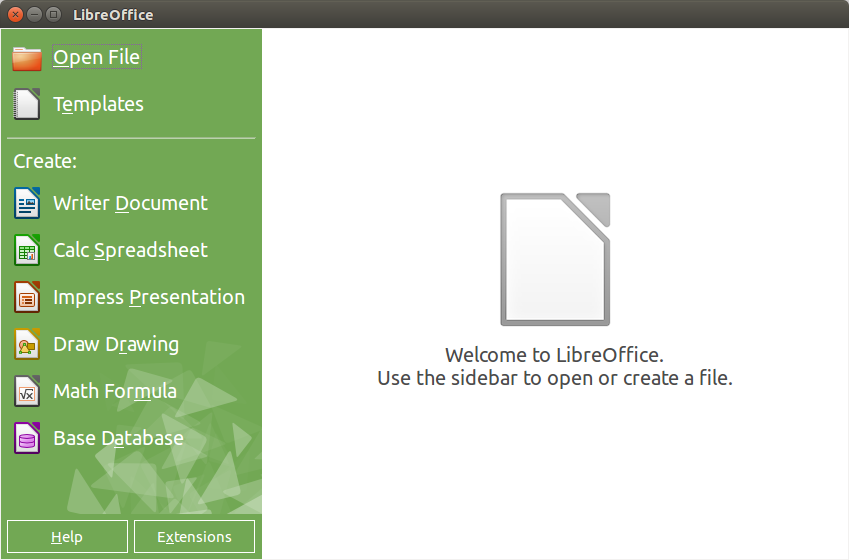
\includegraphics[scale=0.46]{pics/40.png}
\end{center}

لیبره آفیس از بخش‌های زیر تشکیل می‌شود:
\begin{itemize}
\item \lr{\textbf{Writer}}: برنامه‌ای است برای نوشتن و ویرایش متن. این نرم‌افزار زبان فارسی را کاملاً پشتیبانی می‌کند. خروجی پیش‌فرض آن \lr{odt} است، اما می‌توانید خروجی‌هایی مانند \lr{doc} و \lr{pdf} نیز داشته باشید.
\item \lr{\textbf{Impress}}: نرم‌افزار ساخت فایل‌های ارائه که معادل \lr{PowerPoint} در مجموعهٔ آفیس مایکروسافت است.
\item \lr{\textbf{Calc}}: این نرم‌افزار برای ساخت و ویرایش فایل‌های صفحه‌گسترده است.
\item \lr{\textbf{Draw}}: برای طراحی‌های سادهٔ گرافیکی مورد استفاده قرار می‌گیرد.
\item \lr{\textbf{Base}}: نرم افزاری برای طراحی مفهومی پایگاه‌داده و روابط بین جداول است و عملکردی مانند \lr{MS Access} و \lr{Power Designer} دارد.
\item \lr{\textbf{Math}}: کار نوشتن فرمول‌های ریاضی را انجام می‌دهد.
\end{itemize}

\subsection[Gimp]{\lr{Gimp}}

\begin{center}
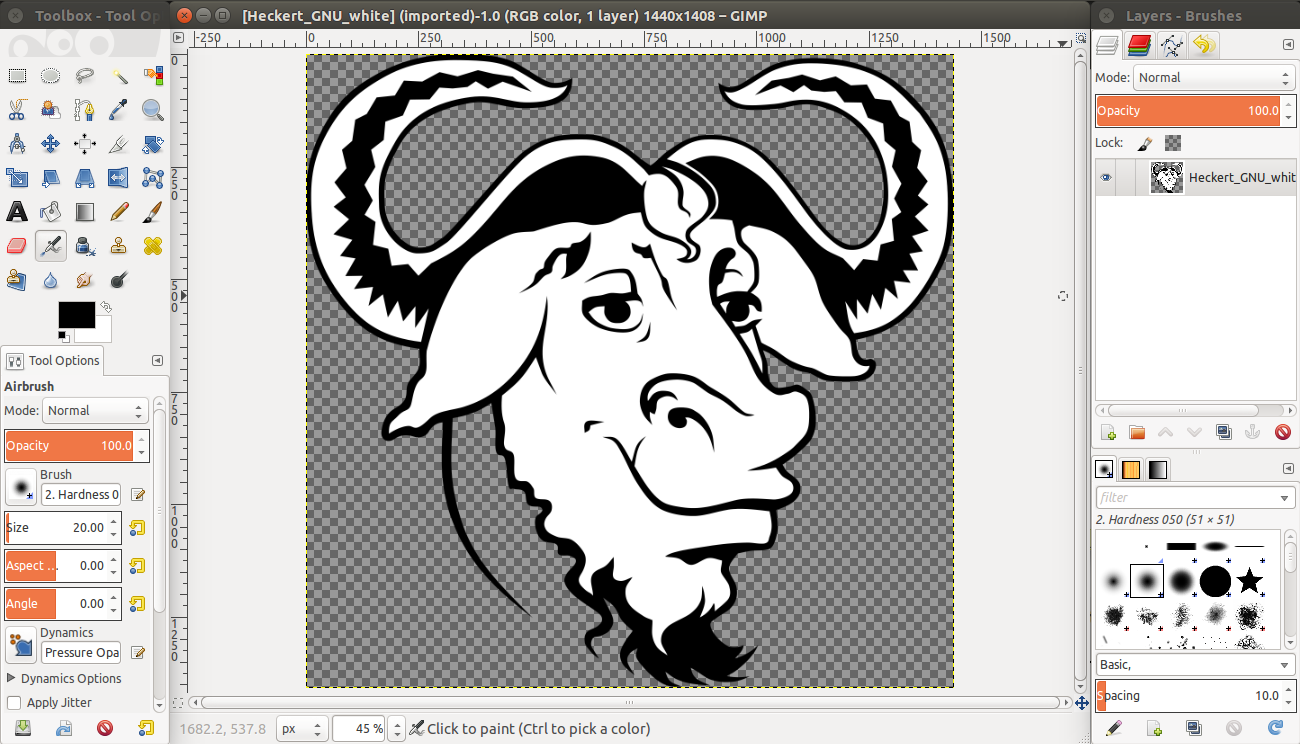
\includegraphics[scale=0.36]{pics/41.png}
\end{center}

نرم‌افزاری است که برای طراحی‌های گرافیکی و ویرایش تصاویر استفاده می‌شود و تا حدودی شبیه \lr{Photoshop} است. از فایل‌های \lr{psd} نیز پشتیبانی می‌کند. \lr{Gimp} ابزارها و فیلترهای متنوعی برای ویرایش تصاویر دارد که به ساخت تصاویری زیبا کمک می‌کند.

\subsection[Inkscape]{\lr{Inkscape}}

\begin{center}
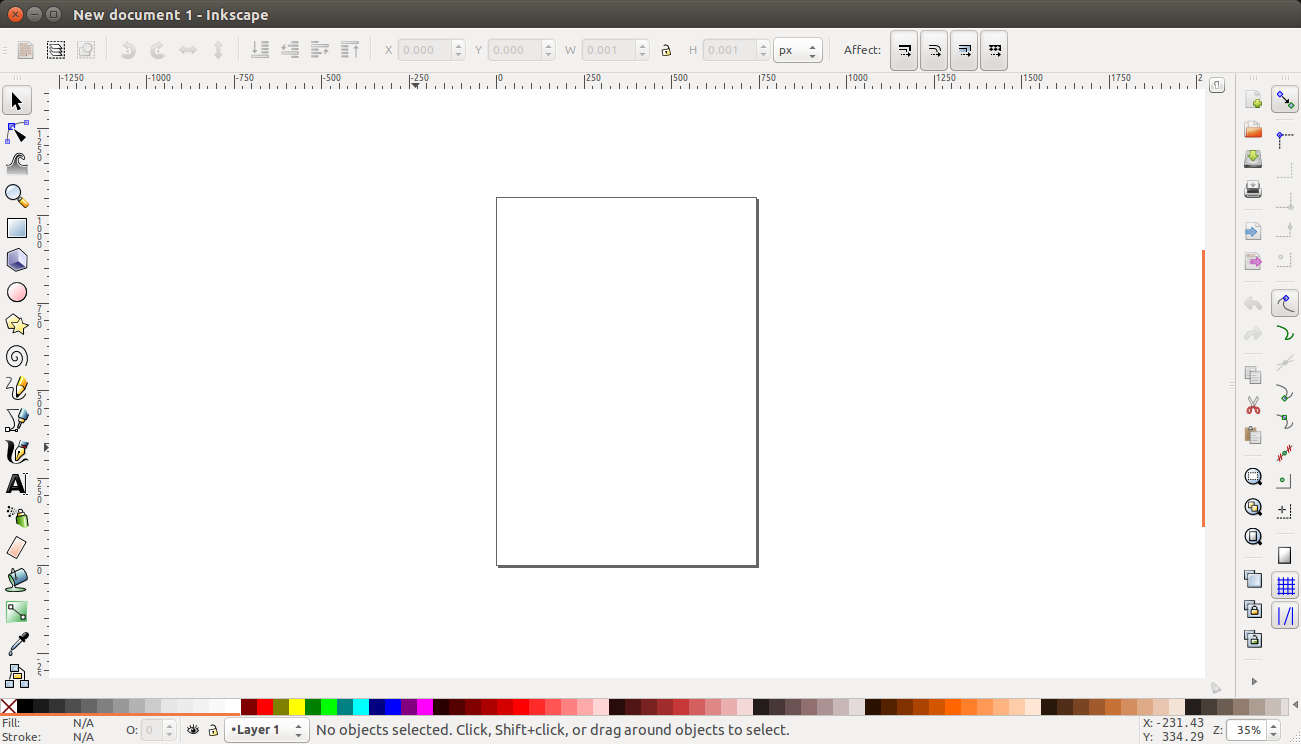
\includegraphics[scale=0.3]{pics/42.png}
\end{center}

یکی از حرفه‌ای‌ترین نرم‌افزارها در زمینه طراحی تصاویر بُرداری (\lr{vector}) است. بسیاری از طرح‌ها و آیکن‌های موجود در اوبونتو با این نرم‌افزار طراحی شده‌اند. \lr{Inkscape} جایگزین مناسبی برای نرم‌افزار \lr{illustrator} به حساب می‌آید.

\subsection[Blender]{\lr{Blender}}

\begin{center}
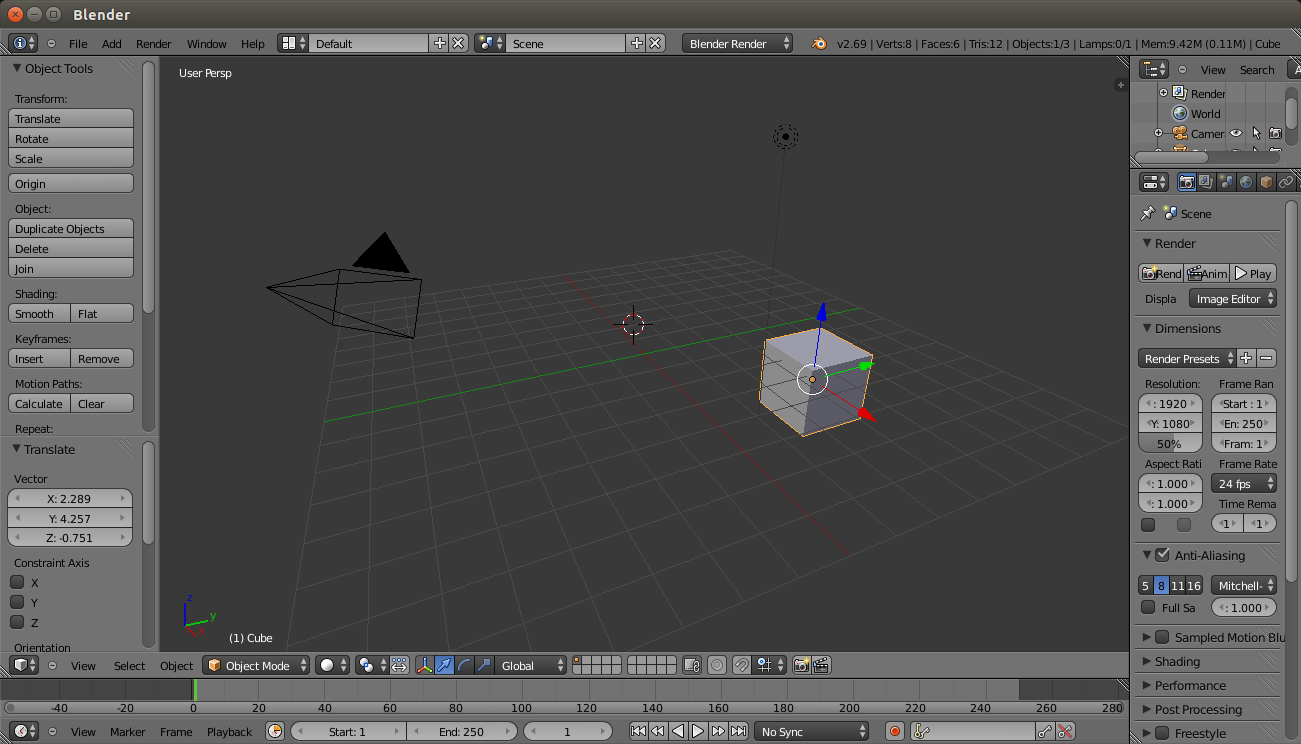
\includegraphics[scale=0.3]{pics/43.png}
\end{center}

این نرم‌افزار برای تمامی طراحان سه‌بعدی دنیای کامپیوتر توصیه می‌شود. \lr{Blender} نرم‌افزاری است که در بسیاری از فیلم‌های هالیوودی و بازی‌های کامپیوتری معروف استفاده شده است و همچنین انیمیشن‌های زیادی با این نرم‌افزار ساخته شده است.

\subsection[K3b]{\lr{K3b}}

\begin{center}
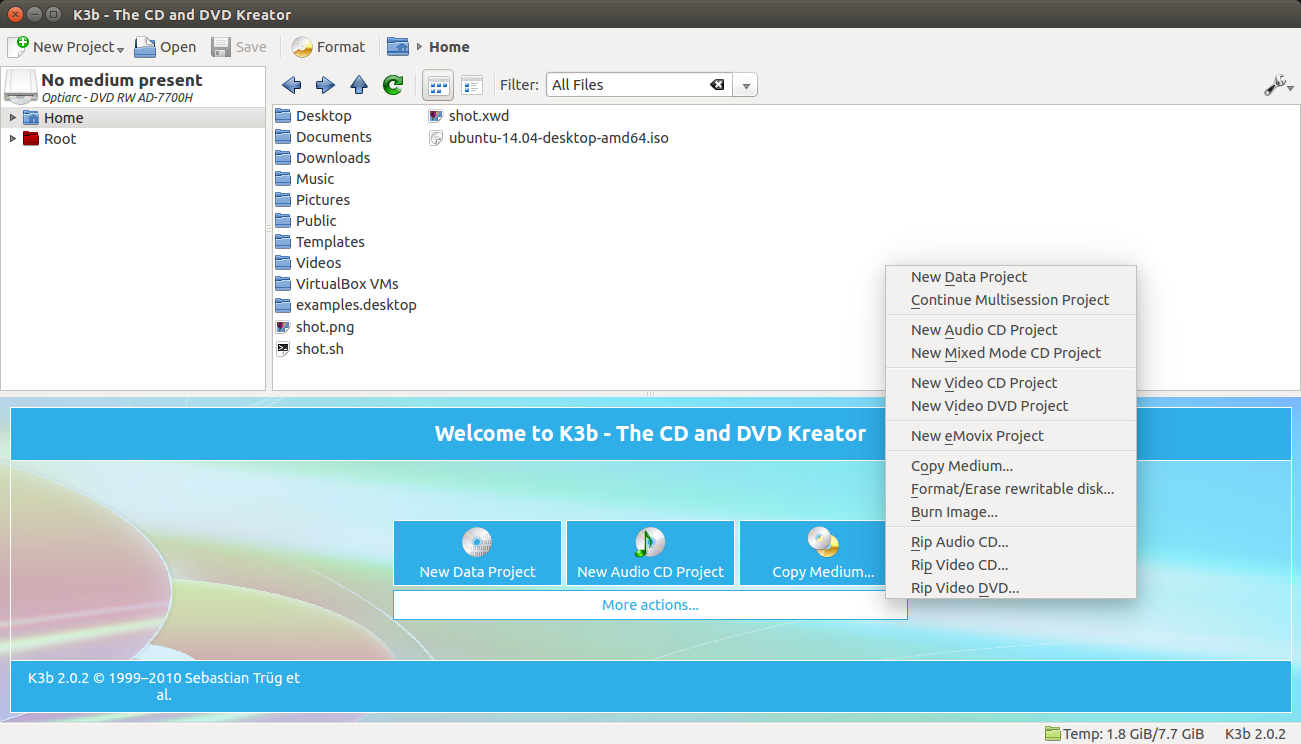
\includegraphics[scale=0.3]{pics/44.png}
\end{center}

نرم‌افزاری برای کپی‌برداری از \lr{CD} و \lr{DVD} است. \lr{K3b} بدون شک یکی از بهترین نرم‌افزارهای موجود در این زمینه است.

\subsection[Darktable]{\lr{Darktable}}

\begin{center}
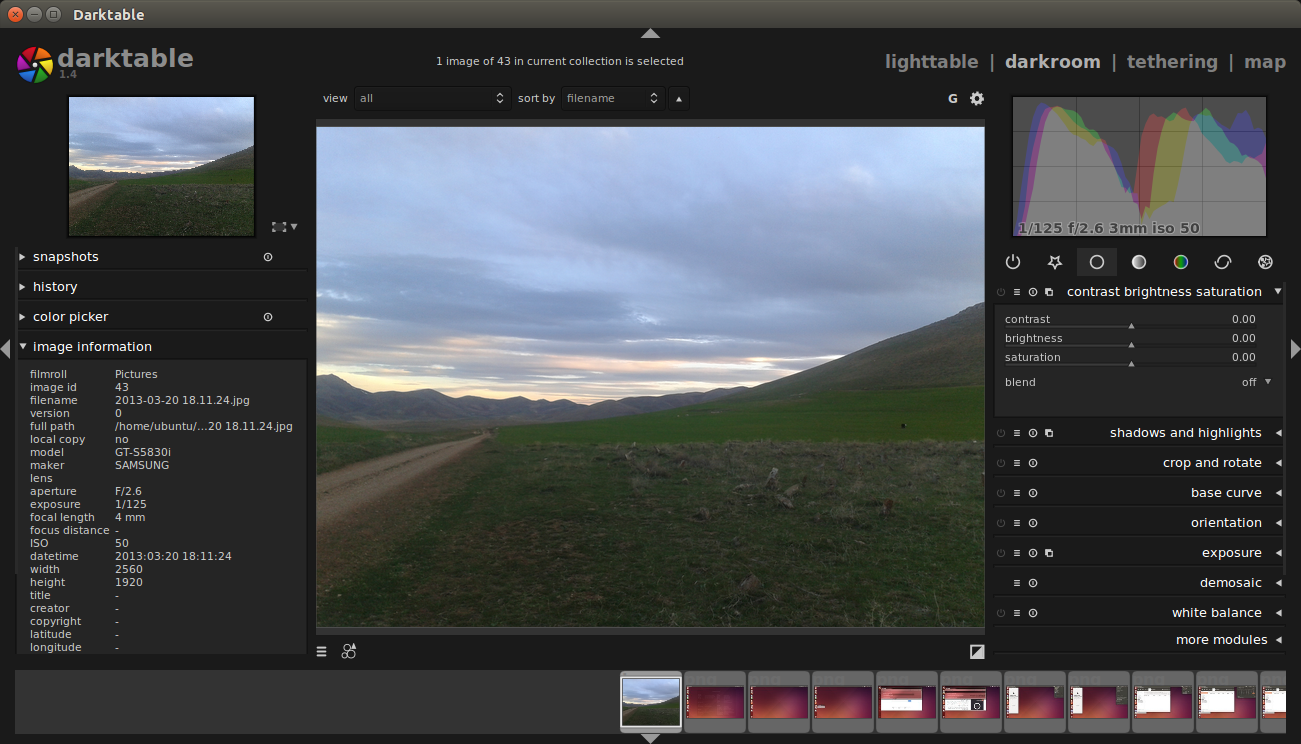
\includegraphics[scale=0.3]{pics/45.png}
\end{center}

چه یک عکاس حرفه‌ای باشید و چه یک کاربر سادهٔ کامپیوتر، با عکس سر و کار خواهید داشت. مهم نیست این عکس‌ها با دوربین حرفه‌ای گرفته می‌شوند یا با دوربین تلفن‌همراه‌تان، مهم نیست که این عکس‌ها از دل طبیعت گرفته شده‌اند یا عکس‌هایی خانوادگی هستند؛ تمامی این عکس‌ها احتیاج به مدیریت و ویرایش در میزان رنگ و روشنی تصویر یا تغییراتی از این دست دارند. \lr{Darktable} تمامی چنین نیازهایی را پاسخ خواهد داد.

\subsection[Virtualbox]{\lr{Virtualbox}}

\begin{center}
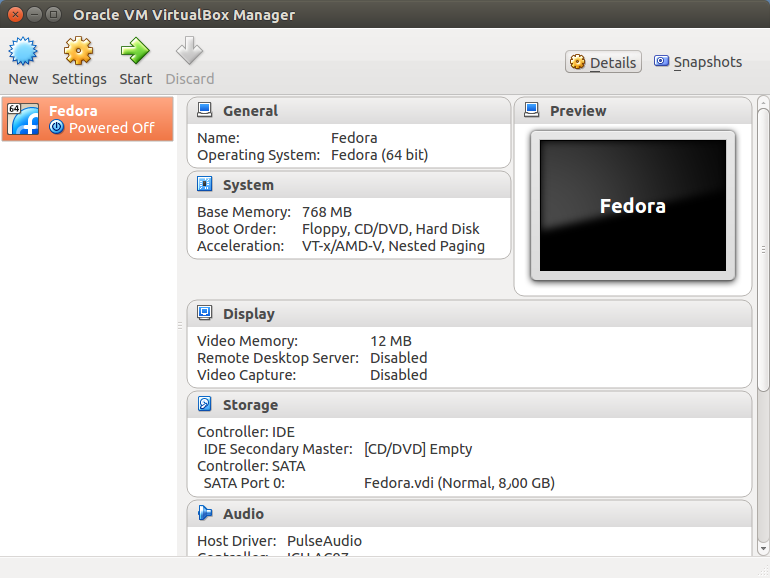
\includegraphics[scale=0.4]{pics/46.png}
\end{center}

با کمک این نرم‌افزار شما قادر خواهید بود که در اوبونتو سیستم عامل دیگری مانند ویندوز را نصب کنید و با اختصاص منابع سیستمی به آن، می‌توانید کاملاً از آن سیستم عامل و نرم‌افزارهایی که روی آن نصب کرده‌اید، استفاده کنید.

\subsection[Wine]{\lr{Wine}}

\begin{center}
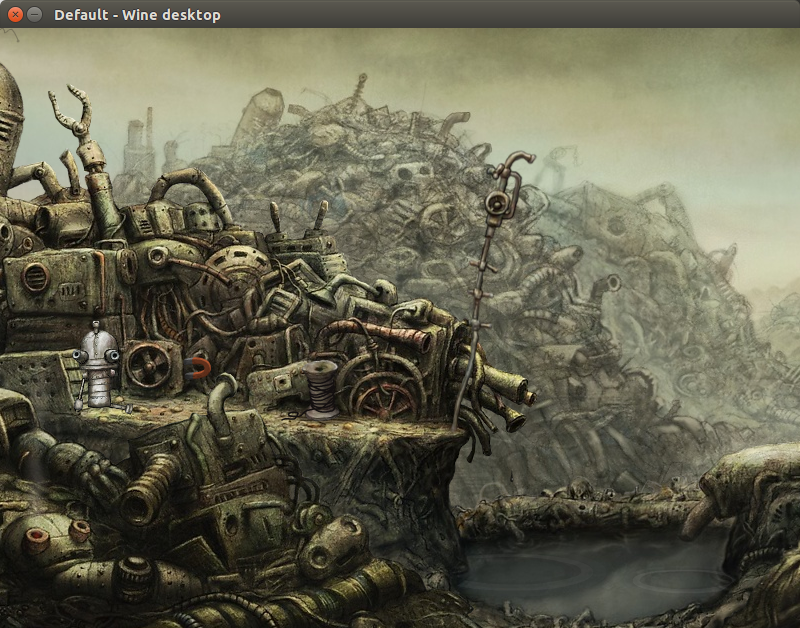
\includegraphics[scale=0.4]{pics/47.png}
\end{center}

معمولاً در اوایل دوران کوچ به سیستم عامل دیگر، زمان‌هایی پیش می‌آید که به نرم‌افزارهای سیستم عامل قبلی خود نیاز پیدا کنید و به دلیل آشنا نبودن با نرم‌افزارهای جایگزین موجود، شاید در ابتدا کار با سیستم عامل جدید کمی آزار‌دهنده باشد. \lr{Wine} نرم‌افزاری است که به شما امکان اجرای بسیاری از نرم‌افزارها و بازی‌های سیستم عامل ویندوز را روی اوبونتو می‌دهد.

\subsection[Goldendict]{\lr{Goldendict}}

\begin{center}
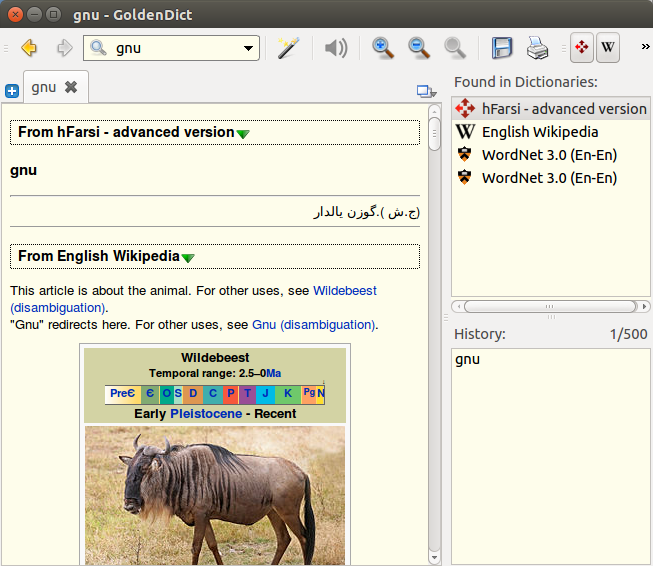
\includegraphics[scale=0.39]{pics/48.png}
\end{center}

وجود یک واژه‌نامه در رایانه نیازی است که کاربران کم‌سن‌وسال تا استادان زبان را شامل می‌شود. \lr{Goldendict} یک برنامهٔ تمام‌عیار برای این نیاز است. این برنامه از کتاب‌خانه لغات \lr{Babylon} با قالب \lr{bgl} نیز پشتیبانی می‌کند.

\subsection[VLC]{\lr{VLC}}

\begin{center}
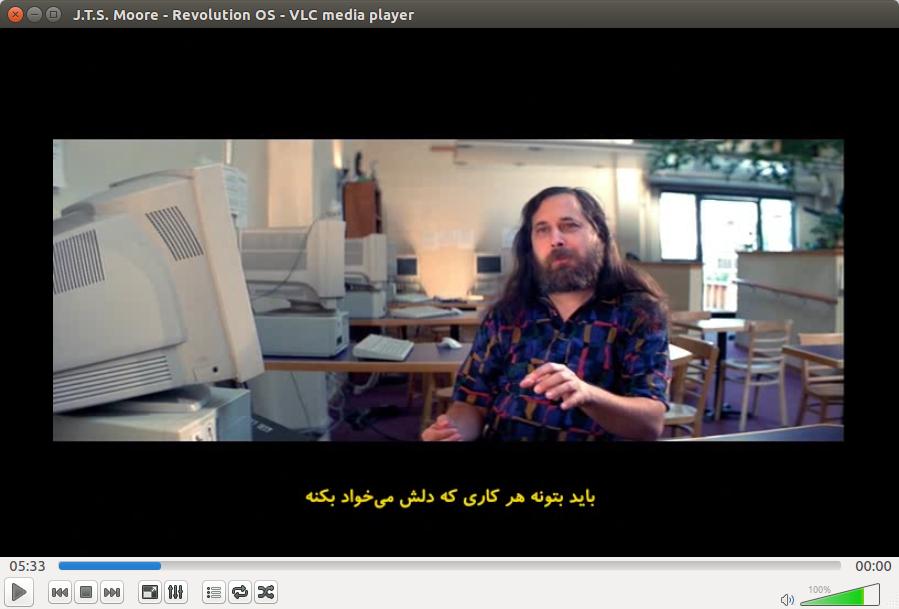
\includegraphics[scale=0.39]{pics/49.png}
\end{center}

شاید با \lr{VLC} در سیستم عامل‌های دیگر نیز کار کرده باشید. \lr{VLC} در زمینهٔ پخش فایل‌های موسیقی و ویدیویی همه‌فن‌حریف است و از بیش‌تر فرمت‌ها، از \lr{MP3} گرفته تا \lr{Bluray}، پشتیانی می‌کند.

\section{نرم‌افزارهای معادل}
از تمام مزایای لینوکس مثل آزادی که بگذریم، شما در گنو/لینوکس هم باید کارهای متداول خود را انجام بدهید. در لیست زیر، نرم‌افزارهای گنو/لینوکسی معادل نرم‌افزارهای پرکاربرد در ویندوز و \lr{Mac OS X} معرفی می‌شوند.\\

\begin{table}[ht]
\caption{لیست نرم‌افزارهای معادل}
\centering
\begin{tabular}{|c|c|}
\hline
\textbf{\lr{\Large Ubuntu}} & \textbf{\lr{\Large Windows / Mac OS X}} \\[1ex]
\hline
\lr{Pinta} & \lr{Paint}\\
\hline
\lr{VLC} & \lr{KMPlayer}\\
\hline
\lr{Totem} & \lr{Windows Media Player}\\
\hline
\lr{Gimp} & \lr{Photoshop}\\
\hline
\lr{OpenShot, PiTiVi} & \lr{Windows Media Player}\\
\hline
\lr{Rhythmbox, Noise} & \lr{iTunes}\\
\hline
\lr{gedit} & \lr{Windows Notepad}\\
\hline
\lr{Blender} & \lr{Autodesk 3D Max}\\
\hline
\lr{LibreCAD} & \lr{Autodesk AutoCAD}\\
\hline
\lr{Audacious} & \lr{Winamp}\\
\hline
\lr{Evince} & \lr{Adobe Acrobat Reader}\\
\hline
\lr{Inkscape} & \lr{Adobe Illustrator}\\
\hline
\lr{Scribus} & \lr{Adobe InDesign}\\
\hline
\lr{LibreOffice} & \lr{Microsoft Office, Apple iWork}\\
\hline
\lr{Empathy, Pidgin} & \lr{Yahoo Messenger, Google Talk}\\
\hline
\end{tabular}
\end{table}
